\section{Introduction}

% CHAIN (one line per claim; the word in <> is reused verbatim later)
% 1  BN classifiers lose accuracy under <covariate shift>; <test-time normalization> re-estimates BN statistics on test data, training-free.
% 2  While effective, test batches are often small (streams, edge devices), and <test batch statistics> of few samples are noisy.
% 3  Practice: mu = mu^src + lambda (hat mu - mu^src); lambda = 1 (TBN), n/(n+N) (Prior-BN), 1-alpha (alpha-BN). Planted: lambda depends on a hyperparameter and n only.
% 4  ROOT CAUSE: whether full, prior or fixed, these rules share one design: the <mixing weight> is fixed before the test batch is seen.
% 5  STANDARD: effective statistics should be <adaptive> (follow the shift) and <stable> (not fluctuate with the few samples).
% 6  (i) Stale Source Statistics -> large shift, small weight -> <shift bias>; (ii) Noisy Batch Statistics -> small batch, large weight -> <estimation variance>.
% 7  KEY IDEA = set the mixing weight after seeing the batch, from the batch itself (fixed before -> set after; hyperparameter -> measured).
% 8  CHALLENGE: the ratio of shift to noise needs the noise level, which a batch of one cannot estimate, and the plug-in ratio is itself noisy -> (a) noise from source, (b) James-Stein.
% 9  shift score <-> (i), Stein weight <-> (ii); together adaptive and stable; guarantee: never worse than TBN, close to the oracle weight.
% 10 First/Second/Third/Fourth (cf Section); We highlight that SourceStein is adaptive and stable at no training cost.
% Mapping: Stale Source Statistics / Noisy Batch Statistics <-> shift score / Stein weight <-> Sec 3.2 / 3.3 <-> RQ2 run-ins (shift bias, estimation variance).

\begin{figure}[t]
    \centering
    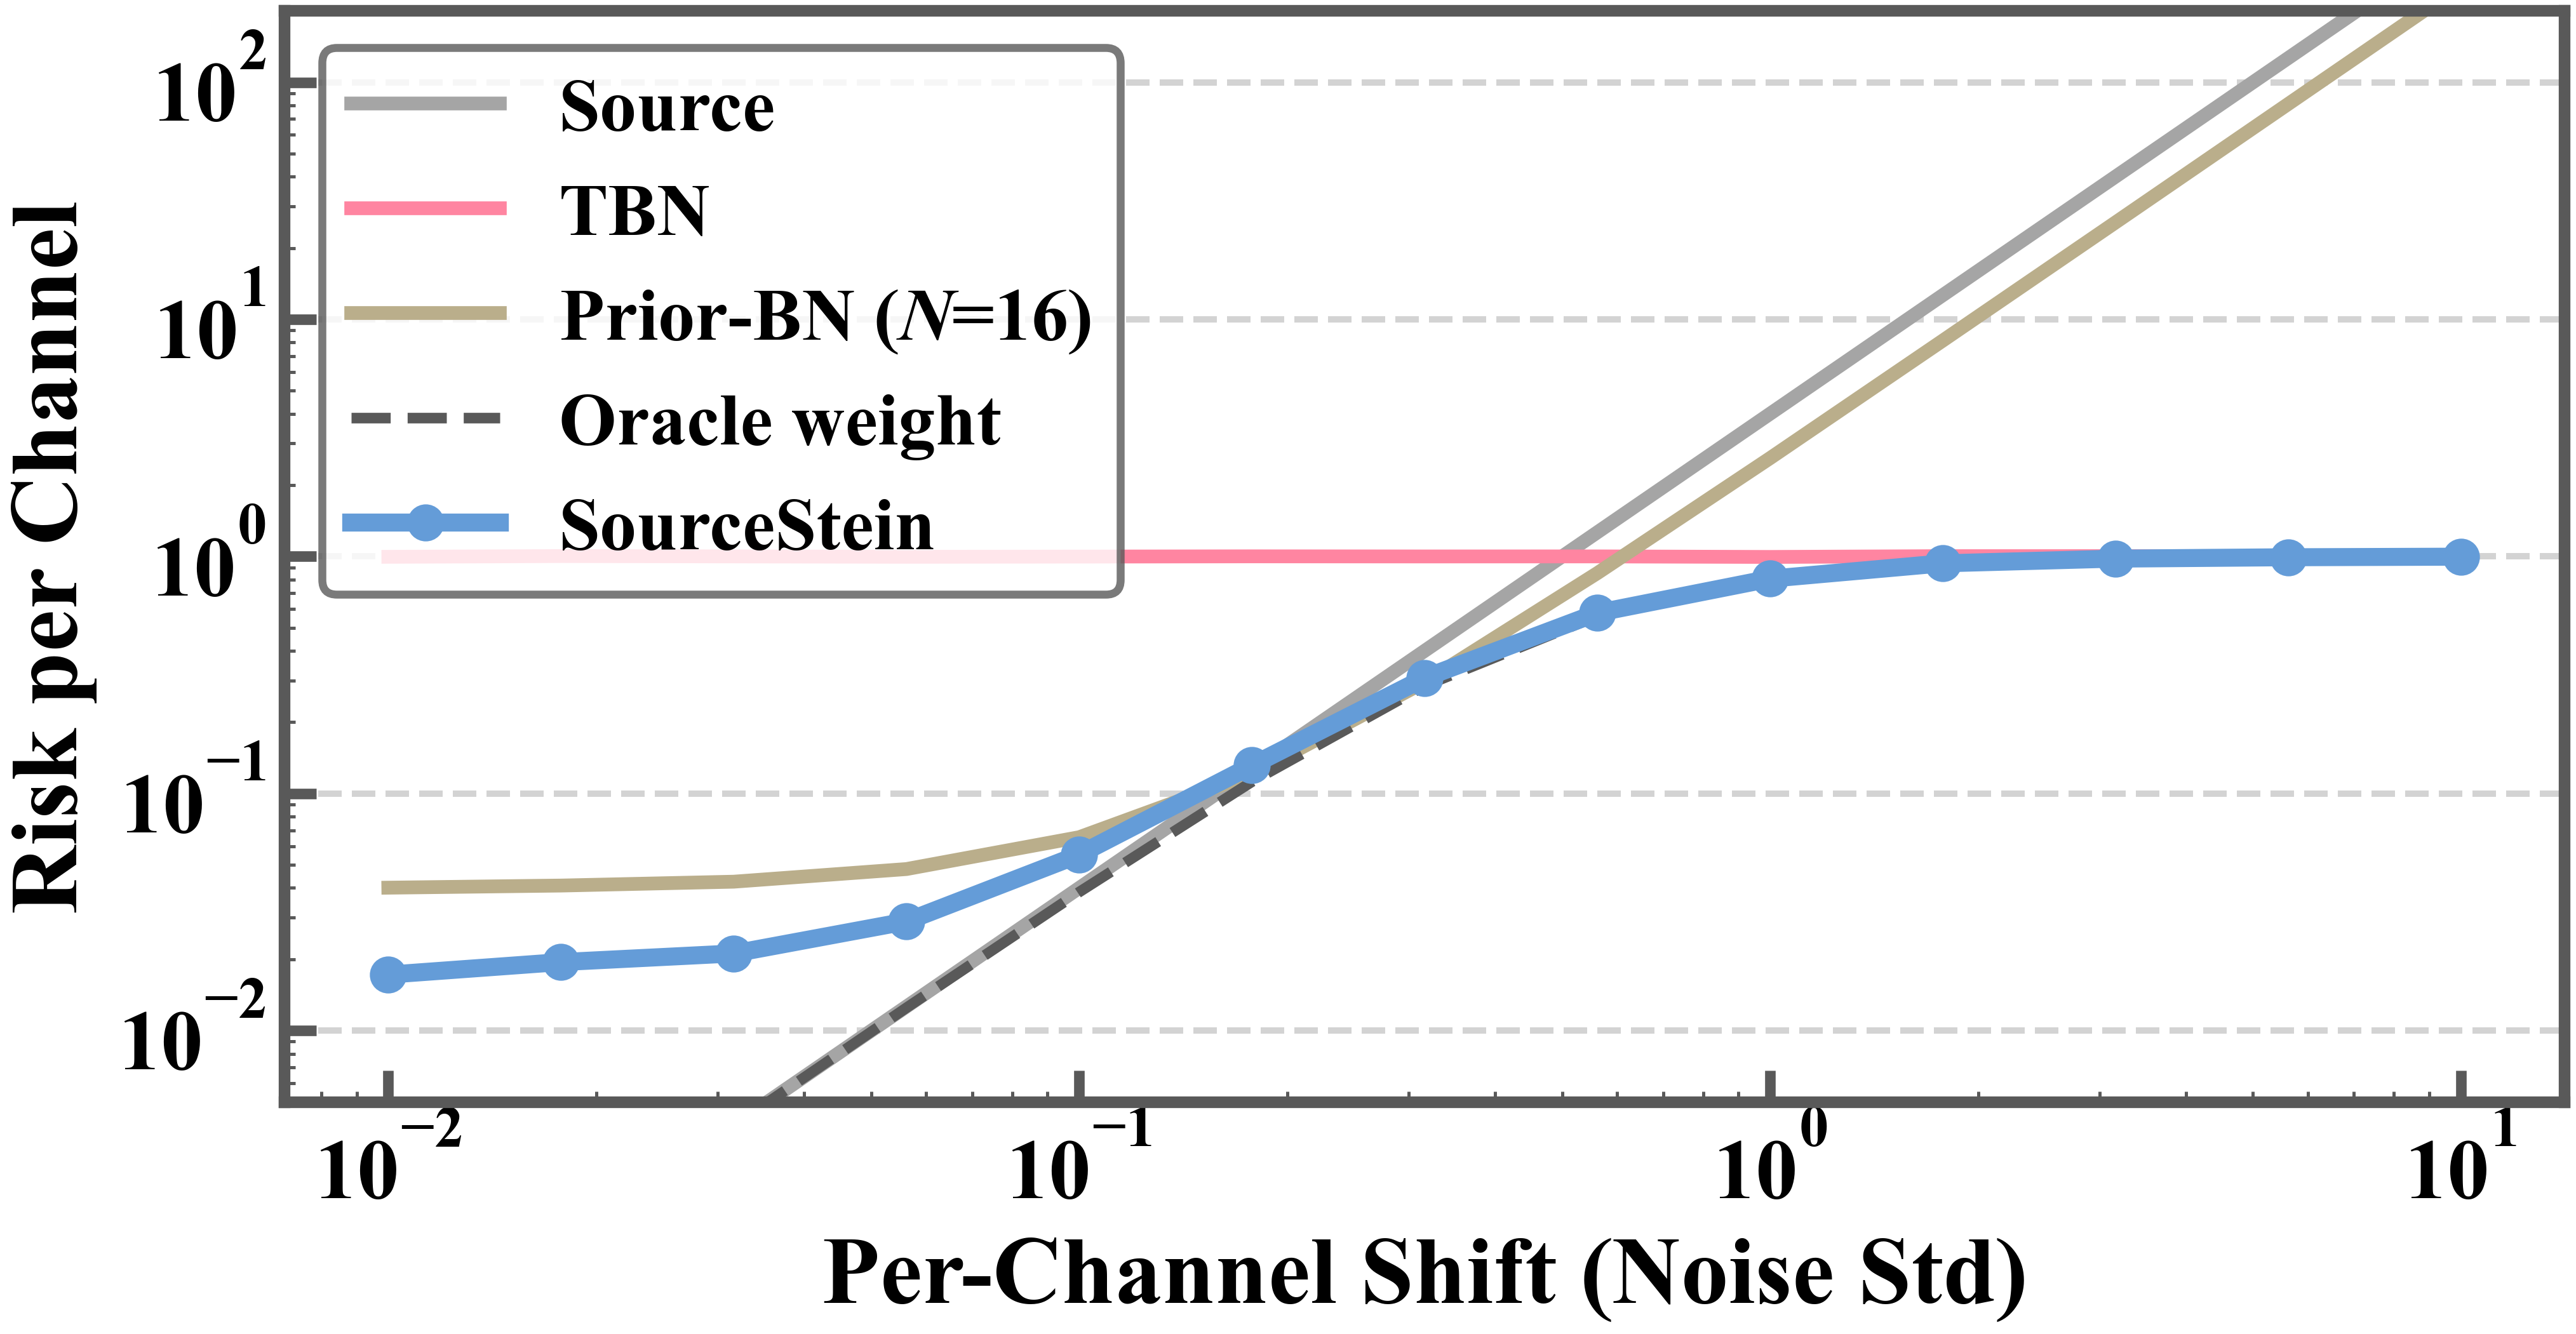
\includegraphics[width=\columnwidth]{figures/exp/synthetic/risk_n4_gauss_s1p0.png}
    \caption{Fixed mixing weights fail at one end of the shift range. Risk of the estimated mean (per channel, in noise units, log scale) for batches of $n{=}4$ simulated samples with $C{=}64$ channels, as the shift increases. Source statistics and Prior-BN incur a shift bias that increases with the shift, while TBN incurs the full estimation variance at each shift; SourceStein follows the oracle weight across the range.}
    \label{fig:teaser-figure}
    \vspace{-12pt}
\end{figure}

Batch normalization (BN) \cite{BatchNorm} is part of most convolutional classifiers.
Each BN layer normalizes its features with statistics collected on the training data, which ties the whole network to the training distribution.
Under \concept{covariate shift} \cite{BN-Adapt}, such as fog or sensor noise at test time, these statistics no longer match the test features.
As a result, the accuracy of a model trained on clean images decreases sharply \cite{CIFAR10-C}.
\concept{Test-time normalization} \cite{AlphaBN} removes much of this loss by re-estimating the BN statistics on the test data, with no labels and no training \cite{PredictionBN, BN-Adapt}.
Because it changes only the statistics, it applies to any trained BN network and adds almost no computation.
While effective, this fix depends on how many test inputs arrive together: streams and edge devices often deliver a handful of images at a time \cite{NOTE, SAR}, and statistics computed from so few samples are unreliable \cite{BN-Adapt}.

To handle small batches, current methods combine two estimates: the stored \concept{source statistics} \cite{BN-Adapt} and the \concept{test batch statistics} \cite{UnMix-TNS}.
In our notation, a layer normalizes with the mean $\boldsymbol{\mu}^{\text{src}} + \lambda(\hat{\boldsymbol{\mu}} - \boldsymbol{\mu}^{\text{src}})$, where $\hat{\boldsymbol{\mu}}$ is the mean of the $n$ test samples and $\lambda \in [0,1]$ is a \concept{mixing weight} (the variance is treated alike).
TBN \cite{PredictionBN} uses $\lambda{=}1$, Prior-BN \cite{BN-Adapt} uses $\lambda{=}n/(n{+}N)$ with a pseudo sample size $N$, and $\alpha$-BN \cite{AlphaBN} uses a constant $\lambda{=}1{-}\alpha$.
Each choice is set by a hyperparameter and the batch size, and works well in the setting it was tuned for.
These rules have made test-time normalization a strong training-free baseline \cite{TENT}.
Whether full, prior-weighted or constant, these rules share one design: the mixing weight is fixed before the test batch is seen.
Consider a batch of four foggy images (the running example of Figure~\ref{fig:main-figure}): Prior-BN assigns it the same weight $4/(4{+}N)$ as a batch of four clean images, although only the foggy batch has moved away from the training data.

Intuitively, effective test-time statistics should be adaptive (\ie follow the shift of the test data) and stable (\ie not fluctuate with the few samples in a batch).
However, a weight fixed in advance cannot be both.
As shown in Figure~\ref{fig:teaser-figure} on simulated features, this design causes two limitations:
\begin{itemize}[leftmargin=*]
    \item \textbf{Stale Source Statistics.} When the shift is large and the weight is small, the mixed mean remains near the source mean. As a result, the normalization inherits a \concept{shift bias} that increases with the square of the shift. This bias affects Prior-BN most at large $N$, whose weight is in fact optimal for only one shift size (see Section~\ref{sec:shrinkage-problem}).
    \item \textbf{Noisy Batch Statistics.} When the batch is small and the weight is large, the mixed mean copies the sampling noise of $\hat{\boldsymbol{\mu}}$. Consequently, the normalization incurs an \concept{estimation variance} that does not decrease with the shift. This variance makes TBN err on most clean inputs at batch size one (see Table~\ref{tab:clean}).
\end{itemize}

To address these issues, we propose \textbf{SourceStein}, an adaptive and stable rule for test-time normalization.
The key idea is to set the mixing weight after the test batch is seen, from the batch itself, by comparing how far the batch has moved with how far it would move by chance.
In this way, the weight becomes a measurement of each batch rather than a setting chosen before deployment.
However, this comparison requires the noise level of the batch statistics, which a single test image cannot provide.
Moreover, a plug-in estimate of the best weight is itself noisy for small batches \cite{Efron-Morris}.
To this end, we equip each BN layer with two parts.
The first is a \textbf{shift score} $S = n\|\hat{\boldsymbol{\mu}} - \boldsymbol{\mu}^{\text{src}}\|^2_{\boldsymbol{\Sigma}^{-1}}$, which whitens the observed shift with between-sample variances $\boldsymbol{\Sigma}$ stored from the training data.
The second is a \textbf{Stein weight} $\hat{\lambda} = (1 - (C{-}2)/S)_+$ over the $C$ channels of the layer, \ie the positive-part \concept{James--Stein estimator} \cite{James-Stein} with the source statistics as its target.
The shift score keeps the statistics adaptive when the test data have moved, while the Stein weight keeps them stable when the move is within the noise.
Under a Gaussian model, this rule never has a higher risk than TBN and remains close to the best fixed weight for the actual shift.

We then run experiments with two networks on CIFAR-10-C \cite{CIFAR10-C} to test SourceStein.
First, SourceStein generally reduces the error of TBN, Prior-BN and $\alpha$-BN for batches of 1 to 16 images and matches them for larger batches (\cf Section~\ref{sec:main-performance}).
Second, its weight increases with the batch size and with the shift, as the analysis predicts (\cf Section~\ref{sec:mechanism}).
Third, adapting the variance and pooling the score over channels both contribute, and no pseudo sample size of Prior-BN matches SourceStein (\cf Section~\ref{sec:ablation-study}).
Fourth, inside entropy minimization the rule helps one of the two networks (\cf Section~\ref{sec:extension}).
Overall, the rule replaces a hyperparameter that previously had to be tuned on labelled shifted data with a decision made from each batch.
We highlight that SourceStein is adaptive and stable at the cost of two stored vectors per layer and no training.
